\documentclass[]{article}

\usepackage{
	amsmath, 
	amssymb,
	float,
	graphicx,
	bera,
	parskip,
	xcolor,
	colortbl,
	booktabs
}

\usepackage[
backend=biber, 
style=authoryear,
citestyle=apa, 
sorting=ynt]{biblatex}

\addbibresource{}
\graphicspath{ {Images/} }

\title{Assignment 6}
\author{
	Daniel Bok \\
	ESD \\
	1001049 \\
	daniel\_bok@mymail.sutd.edu.sg 
	\and
	Wong Yan Yee\\ 
	ISTD \\
	1001212 \\
	yanyee\_wong@mymail.sutd.edu.sg
	\and
	Clement Tan \\
	ESD \\
	1000948 \\
	clement\_tan@mymail.sutd.edu.sg
}
\date{\today}

\newcommand{\e}{&=}

\begin{document}
	
\maketitle
	
\section{The Bellman-Ford algorithm}

\begin{table}[htbp]
	\centering
	\caption{Bellman Ford Iterations}
	\begin{tabular}{|lcccccc|}
    \toprule
	\rowcolor[rgb]{ .267,  .447,  .769} \textcolor[rgb]{ 1,  1,  1}{\textbf{Time}} & \textcolor[rgb]{ 1,  1,  1}{\textbf{1}} & \textcolor[rgb]{ 1,  1,  1}{\textbf{2}} & \textcolor[rgb]{ 1,  1,  1}{\textbf{3}} & \textcolor[rgb]{ 1,  1,  1}{\textbf{4}} & \textcolor[rgb]{ 1,  1,  1}{\textbf{5}} & \textcolor[rgb]{ 1,  1,  1}{\textbf{6}} \\
	\midrule
	T = 0 & 0     & $\infty$ & $\infty$ & $\infty$ & $\infty$ & $\infty$ \\
	\midrule
	T = 1 & 0     & 4     & 1     & 5     & $\infty$ & 8 \\
	\midrule
	T = 2 & 0     & 4     & 1     & 5     & 6     & 7 \\
	\midrule
	T = 3 & 0     & 4     & 1     & 5     & 6     & 7 \\
	\bottomrule
	\end{tabular}
	\label{tab:bellman-ford}
\end{table}

\section{Statistical multiplexing}

\subsection{Value of $N_d$ without Statistical Multiplexing}
$N_d = \frac{C}{1} + 1 = C + 1$

\subsection{Ideal number of customers with Statistical Multiplexing}

We should choose $N_s$ such that the probability of the network demand at anyone time will be less than the threshold value, $\gamma = 0.01$.

$\sum_{i = N_d + 1}^{N_s} \mathbb{P}(X = i)$ represents the probability that the network is congested at any one time given that it has $N_s$ users.

Given that $p = 0.1$, we have
\begin{align*}
\sum_{i = N_d + 1}^{N_s} \binom{N_s}{i} p^i (1 - p)^{N_s - i} &\leq \gamma
\end{align*}
For different values of $C$, we have
\begin{enumerate}
\item[10] $N_s = 50$
\item[20] $N_s = 122$
\item[30] $N_s = 200$
\end{enumerate}

\subsection{Tale of 2 Systems}

\begin{description}
\item[System A] Double the capacity of link and load or double the users. 
\item[System B] Double the number of links, each receiving the original amount of users
\end{description}

System A can fit a larger amount of users. By utilizing resource pooling, its larger capacity ensure that the probability that all users will demand capacity beyond the single maximum level is smaller than the probability that 2 such systems (with half the bandwidth) will hit the maximum capacity. Another way to see this is to understand that by statistical multiplexing, the chances of System A hitting congestion is lower than the System B.

\section{Load and Erlang formula}

\begin{figure}[H]
\centering
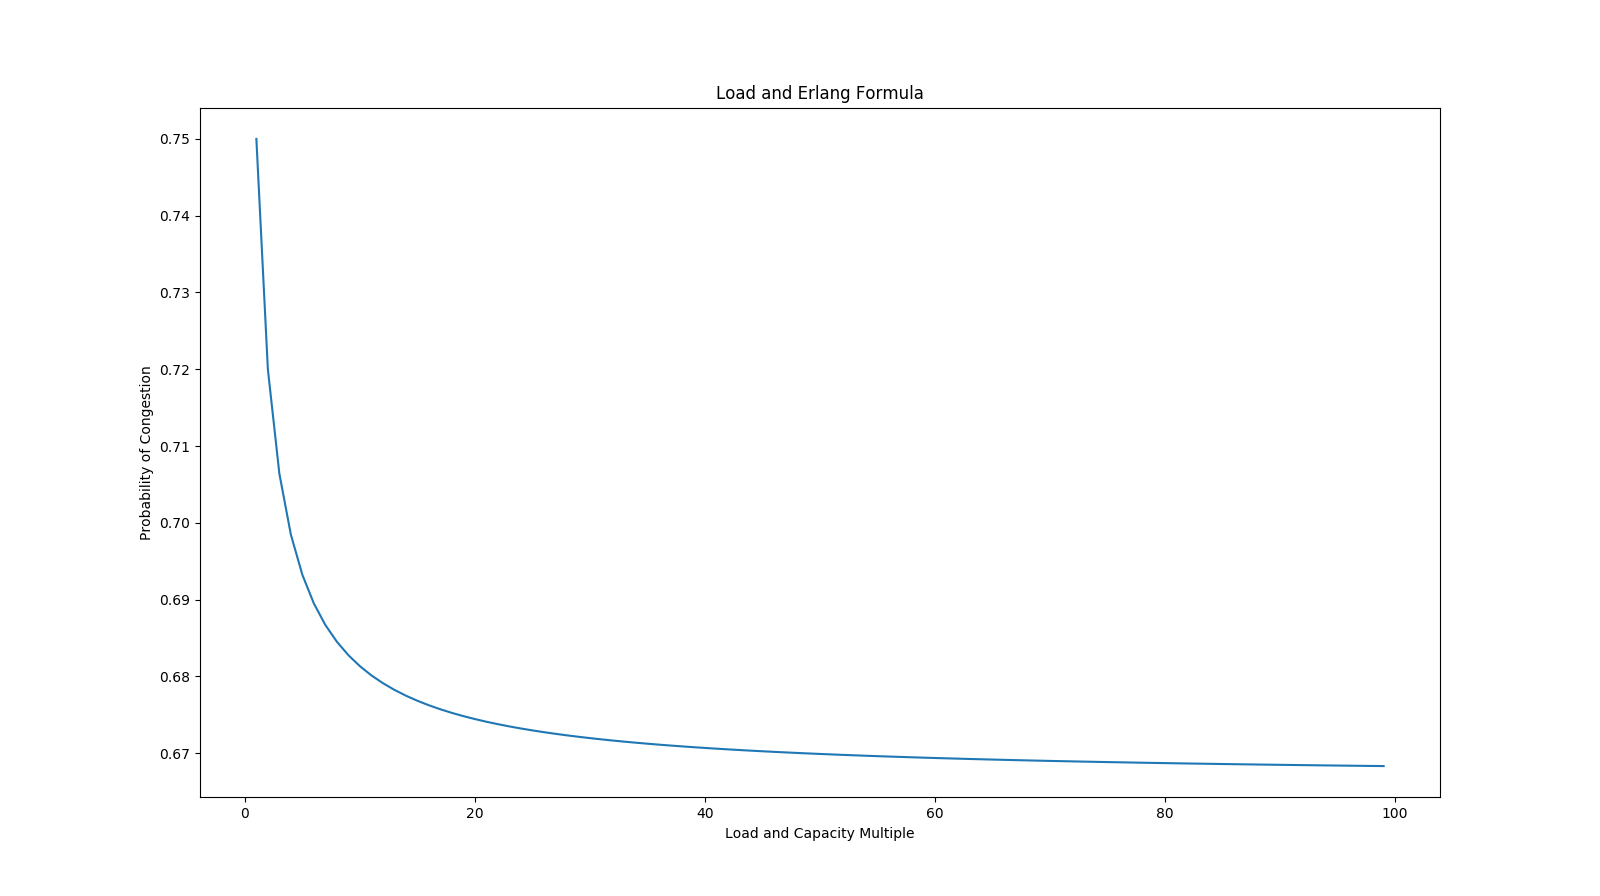
\includegraphics[width=\linewidth]{figure-1.png}
\caption{Probability of congestion given increasing load and capacity multiples}
\label{fig:LEF}
\end{figure}

We see from Figure \ref{fig:LEF} that by increasing the multiples on the load and capacity, the probability of congestion decreases (resource pooling) and will eventually converge.

This shows that
\begin{gather*}
E[tn, t\rho] \leq E[n, \rho] \quad \forall (t > 1)
\end{gather*}

\end{document}
